% ===================================================================
%  Week 5 — Session 2: Canny, thresholds & clean contours
% ===================================================================
\documentclass[10pt,aspectratio=169]{beamer}
% ===================================================================
%  Shared Beamer preamble for "Practical Image Processing"
%  English slides. Compile with pdfLaTeX.
% ===================================================================

\usetheme{metropolis}
\usepackage[T1]{fontenc}
\usepackage[utf8]{inputenc}
\usepackage{lmodern}
\usepackage{listings}
\usepackage{tcolorbox}
\usepackage{fontawesome5}
\usepackage{booktabs}
\usepackage{amsmath,amssymb}
\usepackage{tikz}
\usepackage{pgfplots}
\pgfplotsset{compat=1.17}
\usetikzlibrary{arrows.meta,positioning,shapes.geometric,fit,backgrounds,matrix}
\tcbuselibrary{skins,breakable}

% ---- Palette --------------------------------------------------------
\definecolor{coursePrimary}{HTML}{1B4965}   % deep blue
\definecolor{courseAccent}{HTML}{E76F51}    % coral
\definecolor{courseGood}{HTML}{2A9D8F}      % teal
\definecolor{courseBad}{HTML}{C0392B}       % red
\definecolor{courseInfo}{HTML}{2980B9}      % blue
\definecolor{codeBg}{HTML}{F5F6FA}
\definecolor{codeKw}{HTML}{8E44AD}
\definecolor{codeStr}{HTML}{2A9D8F}
\definecolor{codeCom}{HTML}{7F8C8D}

\setbeamercolor{frametitle}{bg=coursePrimary}
\setbeamercolor{progress bar}{fg=courseAccent}
\setbeamercolor{alerted text}{fg=courseAccent}
\metroset{block=fill,sectionpage=progressbar,numbering=fraction}

% ---- Code listings (Python is built into listings) -----------------
\lstdefinestyle{course}{
  backgroundcolor=\color{codeBg},
  basicstyle=\ttfamily\scriptsize,
  keywordstyle=\color{codeKw}\bfseries,
  stringstyle=\color{codeStr},
  commentstyle=\color{codeCom}\itshape,
  numberstyle=\tiny\color{codeCom},
  numbers=left, numbersep=6pt,
  showstringspaces=false, breaklines=true, breakatwhitespace=true,
  tabsize=4, columns=fullflexible,
  frame=single, framesep=4pt, rulecolor=\color{gray!30},
  keepspaces=true, upquote=true, language=Python,
}
\lstset{style=course}
\lstdefinelanguage{bash}{
  keywords={cd,pip,python,venv,source,import}, sensitive=true,
  morecomment=[l]{\#}, morestring=[b]', morestring=[b]",
}

% ---- Reusable callout boxes ----------------------------------------
\newtcolorbox{goodbox}[1][Good practice]{colback=courseGood!8,colframe=courseGood,
  fonttitle=\bfseries,title={\faCheck~#1},boxrule=0.6pt,left=4pt,right=4pt,top=3pt,bottom=3pt}
\newtcolorbox{badbox}[1][Pitfall]{colback=courseBad!8,colframe=courseBad,
  fonttitle=\bfseries,title={\faTimes~#1},boxrule=0.6pt,left=4pt,right=4pt,top=3pt,bottom=3pt}
\newtcolorbox{infobox}[1][Note]{colback=courseInfo!8,colframe=courseInfo,
  fonttitle=\bfseries,title={\faInfoCircle~#1},boxrule=0.6pt,left=4pt,right=4pt,top=3pt,bottom=3pt}
\newtcolorbox{mathbox}[1][Math]{colback=coursePrimary!6,colframe=coursePrimary,
  fonttitle=\bfseries,title={\faCalculator~#1},boxrule=0.6pt,left=4pt,right=4pt,top=3pt,bottom=3pt}

\newcommand{\keyidea}[1]{\begin{alertblock}{Key idea}#1\end{alertblock}}
\newcommand{\term}[1]{\textbf{\color{coursePrimary}#1}}
\newcommand{\code}[1]{\lstinline[basicstyle=\ttfamily\small]|#1|}

% ---- A helper to draw a small pixel grid, cells shaded by value ----
% \pixelgrid{ {10,20,120,200,240}, {30,60,130,180,230}, ... }
\newcommand{\pixelgrid}[1]{%
  \begin{tikzpicture}[font=\scriptsize,scale=0.6]
    \foreach \row [count=\ry] in {#1} {
      \foreach \val [count=\cx] in \row {
        \draw[gray,fill=coursePrimary!8] (\cx,-\ry) rectangle ++(1,-1);
        \node at (\cx+0.5,-\ry-0.5) {\val};
      }
    }
  \end{tikzpicture}}


\title{Edge Detection}
\subtitle{Week 5 — Session 2: Canny, thresholds \& clean contours}
\author{Practical Image Processing}
\date{Lecture 5.2 \textbullet\ 60--70 min}

\begin{document}

\maketitle

\begin{frame}{Recap of Session 1}
  \begin{columns}[T]
    \begin{column}{0.6\textwidth}
      \begin{itemize}
        \item An edge $=$ a large \term{gradient}; we built \term{Sobel}/\term{Prewitt}/\term{Scharr}.
        \item Magnitude $\sqrt{g_x^2+g_y^2}$ (strength) and direction $\operatorname{atan2}(g_y,g_x)$.
        \item \term{Laplacian}/\term{LoG} for zero-crossings; always \term{smooth before differentiating}.
      \end{itemize}
    \end{column}
    \begin{column}{0.4\textwidth}
      \begin{alertblock}{Today (Session 2)}
        The thresholded Sobel magnitude is thick and broken. We turn it into thin, connected
        contours with the \term{Canny} detector, then feed DocScan.
      \end{alertblock}
    \end{column}
  \end{columns}
\end{frame}

\begin{frame}{Roadmap — Session 2}\tableofcontents\end{frame}

% ==================================================================
\section{Why a raw gradient isn't enough}
% ==================================================================

\begin{frame}{The problem with thresholded magnitude}
  \begin{itemize}
    \item Threshold too low $\Rightarrow$ noise everywhere; too high $\Rightarrow$ real edges break up.
    \item Edges come out \term{several pixels thick} — the gradient ramps up and down across the edge.
    \item Edges are \term{broken}: intensity dips below threshold along a real contour.
  \end{itemize}
  \begin{badbox}
    One global threshold can never be both sensitive (catch faint edges) and clean (reject noise)
    at the same time. We need something smarter.
  \end{badbox}
\end{frame}

\begin{frame}{Canny: the gold-standard pipeline}
  \begin{center}
  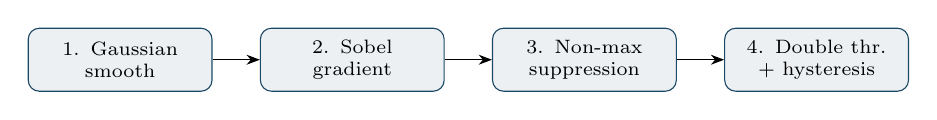
\begin{tikzpicture}[font=\scriptsize,node distance=6mm,
    box/.style={draw=coursePrimary,fill=coursePrimary!8,rounded corners,
      minimum height=8mm,text width=2.1cm,align=center},>=Stealth]
    \node[box](s1){1. Gaussian\\smooth};
    \node[box,right=of s1](s2){2. Sobel\\gradient};
    \node[box,right=of s2](s3){3. Non-max\\suppression};
    \node[box,right=of s3](s4){4. Double thr.\\+ hysteresis};
    \draw[->](s1)--(s2); \draw[->](s2)--(s3); \draw[->](s3)--(s4);
  \end{tikzpicture}
  \end{center}
  \begin{enumerate}
    \item \term{Smooth} with a Gaussian (kill noise).
    \item \term{Gradient} magnitude \& direction (Sobel).
    \item \term{Non-maximum suppression}: thin thick edges to 1-pixel ridges.
    \item \term{Double threshold + hysteresis}: keep strong edges, and weak ones \emph{connected} to strong.
  \end{enumerate}
  \keyidea{Canny is not a kernel — it's a 4-step algorithm producing clean, thin, connected edges.}
\end{frame}

% ==================================================================
\section{Step by step}
% ==================================================================

\begin{frame}{Steps 1--2: smooth, then gradient}
  \begin{itemize}
    \item \term{Step 1 — smooth:} a $5{\times}5$ Gaussian removes the noise that would fake edges
          (Session 1's lesson made concrete).
    \item \term{Step 2 — gradient:} Sobel gives magnitude $M$ and direction $\theta$ at every pixel.
    \item $\theta$ is snapped to one of four directions: $0^\circ, 45^\circ, 90^\circ, 135^\circ$ —
          the neighbours we will compare against in step 3.
  \end{itemize}
  \begin{infobox}
    Steps 1--2 are exactly what you built last session. Canny's novelty is steps 3--4.
  \end{infobox}
\end{frame}

\begin{frame}{Step 3: non-maximum suppression (NMS)}
  \begin{columns}[T]
    \begin{column}{0.52\textwidth}
      \begin{itemize}
        \item A real edge is a \term{ridge} of the magnitude. We keep only the ridge \emph{crest}.
        \item For each pixel, look at the two neighbours \emph{along the gradient direction}.
        \item Keep the pixel only if its magnitude is $\geq$ both. Otherwise set it to 0.
        \item Result: the multi-pixel-thick edge collapses to a \term{1-pixel} line.
      \end{itemize}
    \end{column}
    \begin{column}{0.48\textwidth}
      \begin{center}
      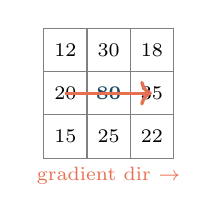
\begin{tikzpicture}[font=\scriptsize,scale=0.55]
        \foreach \x in {0,1,2} \foreach \y in {0,1,2}
          \draw[gray] (\x,\y) rectangle ++(1,1);
        \node at (0.5,1.5){20}; \node[coursePrimary]at(1.5,1.5){\textbf{80}}; \node at(2.5,1.5){35};
        \node at (0.5,2.5){12}; \node at(1.5,2.5){30}; \node at(2.5,2.5){18};
        \node at (0.5,0.5){15}; \node at(1.5,0.5){25}; \node at(2.5,0.5){22};
        \draw[courseAccent,very thick,->] (0.5,1.5)--(2.5,1.5);
        \node[courseAccent] at (1.5,-0.4){gradient dir $\to$};
      \end{tikzpicture}
      \end{center}
      $80 > 20$ and $80 > 35$: \term{keep}. If either neighbour were larger, this pixel is
      suppressed.
    \end{column}
  \end{columns}
\end{frame}

\begin{frame}{The four gradient directions for NMS}
  \begin{columns}[T]
    \begin{column}{0.45\textwidth}
      \begin{center}
      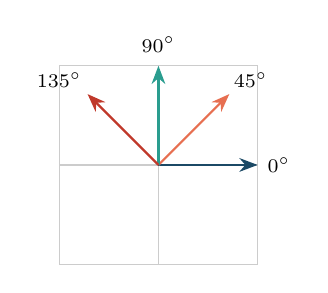
\begin{tikzpicture}[font=\scriptsize,scale=0.9,>=Stealth]
        \draw[gray!40] (-1.4,-1.4) grid[step=1.4] (1.4,1.4);
        \draw[coursePrimary,thick,->] (0,0)--(1.4,0);   \node at (1.7,0){$0^\circ$};
        \draw[courseAccent,thick,->] (0,0)--(1.0,1.0);  \node at (1.3,1.2){$45^\circ$};
        \draw[courseGood,thick,->] (0,0)--(0,1.4);      \node at (0,1.7){$90^\circ$};
        \draw[courseBad,thick,->] (0,0)--(-1.0,1.0);    \node at (-1.4,1.2){$135^\circ$};
      \end{tikzpicture}
      \end{center}
    \end{column}
    \begin{column}{0.55\textwidth}
      \begin{itemize}
        \item The continuous angle $\theta$ is \term{snapped} to the nearest of $0/45/90/135^\circ$.
        \item That fixes which two neighbours to compare against in NMS (the pixels straddling the ridge).
        \item Example: $\theta = 53^\circ$ (Session 1) snaps to $45^\circ$ $\Rightarrow$ compare the two diagonal neighbours.
      \end{itemize}
    \end{column}
  \end{columns}
  \begin{infobox}
    Snapping to 4 bins keeps NMS a simple neighbour lookup instead of a costly interpolation.
  \end{infobox}
\end{frame}

\begin{frame}{Step 4: double threshold + hysteresis}
  \begin{itemize}
    \item Two thresholds: \term{high} $T_H$ (definitely an edge) and \term{low} $T_L$ (maybe).
    \item $M \geq T_H$: \term{strong}. $T_L \leq M < T_H$: \term{weak}. $M < T_L$: \term{drop}.
    \item \term{Hysteresis:} keep every strong edge, plus weak edges \emph{connected} to a strong one; discard isolated weak pixels.
  \end{itemize}
  \begin{goodbox}
    Hysteresis bridges small gaps along a true edge while rejecting scattered noise responses —
    it is why Canny gives long, connected contours.
  \end{goodbox}
\end{frame}

\begin{frame}{Hysteresis, visually}
  \begin{center}
  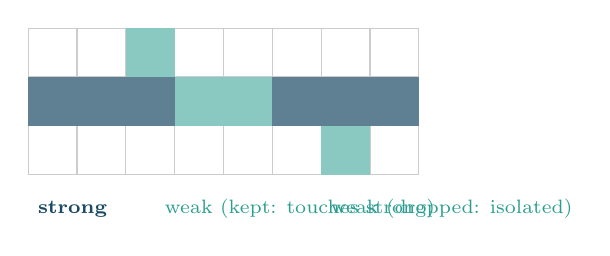
\begin{tikzpicture}[font=\scriptsize,scale=0.62]
    \foreach \x in {0,...,7} \foreach \y in {0,1,2}
      \draw[gray!40] (\x,\y) rectangle ++(1,1);
    % strong chain
    \foreach \x in {0,1,2,5,6,7}
      \fill[coursePrimary!70] (\x,1) rectangle ++(1,1);
    % weak bridging
    \foreach \x in {3,4}
      \fill[courseGood!55] (\x,1) rectangle ++(1,1);
    % isolated weak noise
    \fill[courseGood!55] (2,2) rectangle ++(1,1);
    \fill[courseGood!55] (6,0) rectangle ++(1,1);
    \node[anchor=west,coursePrimary] at (0,-0.7){\textbf{strong}};
    \node[anchor=west,courseGood] at (2.6,-0.7){weak (kept: touches strong)};
    \node[anchor=west,courseGood] at (6.0,-0.7){weak (dropped: isolated)};
  \end{tikzpicture}
  \end{center}
  \begin{itemize}
    \item The weak pixels at $x=3,4$ \term{link} two strong runs $\Rightarrow$ kept.
    \item The lone weak pixels (top-left, bottom-right) touch no strong edge $\Rightarrow$ dropped.
  \end{itemize}
\end{frame}

% ==================================================================
\section{Canny in practice}
% ==================================================================

\begin{frame}{Canny on real images}
  \begin{columns}[T]
    \begin{column}{0.5\textwidth}\begin{center}
      
\includegraphics[width=0.9\linewidth]{../assets/meter_gray.png}\\{\scriptsize meter}\\[3pt]
      
\includegraphics[width=0.9\linewidth]{../assets/meter_canny.png}\\{\scriptsize Canny edges}
    \end{center}\end{column}
    \begin{column}{0.5\textwidth}\begin{center}
      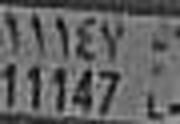
\includegraphics[width=0.7\linewidth]{../assets/plate_gray.png}\\{\scriptsize plate}\\[3pt]
      
\includegraphics[width=0.7\linewidth]{../assets/plate_canny.png}\\{\scriptsize Canny edges}
    \end{center}\end{column}
  \end{columns}
\end{frame}

\begin{frame}[fragile]{Canny in code}
\begin{lstlisting}[language=Python]
blur  = cv2.GaussianBlur(gray, (5, 5), 0)     # step 1: smooth
edges = cv2.Canny(blur, 80, 160)              # low=80, high=160
# OpenCV does steps 2-4 internally: Sobel -> NMS -> hysteresis.
# rule of thumb: high ~= 2-3x low.
\end{lstlisting}
  \begin{itemize}
    \item \code{L2gradient=True} uses the exact $\sqrt{g_x^2+g_y^2}$ (vs the faster $|g_x|+|g_y|$).
    \item \code{apertureSize} is the internal Sobel \code{ksize} (default 3).
  \end{itemize}
\end{frame}

\begin{frame}{The blur matters: with vs without}
  \begin{columns}[T]
    \begin{column}{0.5\textwidth}\begin{center}
      
\includegraphics[width=0.9\linewidth]{../assets/meter_canny_noblur.png}\\
      {\scriptsize Canny \emph{without} pre-blur}
    \end{center}\end{column}
    \begin{column}{0.5\textwidth}\begin{center}
      
\includegraphics[width=0.9\linewidth]{../assets/meter_canny.png}\\
      {\scriptsize Canny \emph{with} $5{\times}5$ blur}
    \end{center}\end{column}
  \end{columns}
  \vspace{2pt}
  \begin{badbox}
    Skipping the blur floods the map with noise edges. The plate shows it too
    (\code{plate\_canny\_noblur} vs \code{plate\_canny}).
  \end{badbox}
\end{frame}

\begin{frame}{Tuning the two thresholds}
  \begin{itemize}
    \item Raise \term{$T_H$}: fewer edges, only the strongest survive — contours may fragment.
    \item Lower \term{$T_L$}: more weak edges get rescued by hysteresis — but noise creeps back.
    \item Keep the ratio $T_H : T_L \approx 2{:}1$ to $3{:}1$; move both together to trade
          sensitivity for cleanliness.
  \end{itemize}
  \begin{infobox}
    Tune on your \emph{hardest} images (shadowed, low-contrast meter photos), not the easy ones.
  \end{infobox}
\end{frame}

\begin{frame}[fragile]{Auto-Canny: thresholds from the median}
\begin{lstlisting}[language=Python]
import numpy as np
def auto_canny(img, sigma=0.33):
    v = np.median(img)
    lo = int(max(0,   (1.0 - sigma) * v))    # ~0.66 * median
    hi = int(min(255, (1.0 + sigma) * v))    # ~1.33 * median
    return cv2.Canny(img, lo, hi)
\end{lstlisting}
  \begin{itemize}
    \item Fixed thresholds fail across lightings; derive them from the image's own median.
    \item A robust starting recipe — then fine-tune \code{sigma} on hard images.
  \end{itemize}
\end{frame}

\begin{frame}{Closing gaps for the next step}
  \begin{itemize}
    \item Even a good Canny contour can have \term{tiny breaks} where contrast dips.
    \item Week 9's contour finder wants a \emph{closed} loop around the page — a 1-pixel gap can split it in two.
    \item Cheap fix: a light \term{dilation} (or a morphological \term{close}) fuses the gap without fattening the whole edge.
  \end{itemize}
  \begin{goodbox}
    Order matters: Canny \emph{first} (thin, clean), then a small close — not a big blur that would
    have smeared the edge away before detection.
  \end{goodbox}
\end{frame}

% ==================================================================
\section{In-class exercise}
% ==================================================================

\begin{frame}{\faPen~In-class exercise (10 min)}
  \begin{infobox}[Trace hysteresis by hand]
  \end{infobox}
  A 1D magnitude row (after NMS): \code{[2, 9, 5, 4, 6, 10, 1]}, with $T_L=4$, $T_H=8$.
  \begin{enumerate}
    \item Label each pixel \term{strong} ($\geq 8$), \term{weak} ($4\text{--}7$), or \term{drop} ($<4$).
    \item Apply hysteresis: which weak pixels survive because they connect to a strong one?
    \item Which pixels are in the final edge map? What changes if $T_L$ drops to 2?
  \end{enumerate}
\end{frame}

\begin{frame}{\faPen~Debrief}
  \begin{itemize}
    \item Labels: \code{[drop, strong, weak, weak, weak, strong, drop]} (indices 1 and 5 are strong).
    \item The weak run at indices 2--4 is bracketed by strong pixels (1 and 5) $\Rightarrow$ all kept by hysteresis.
    \item Final edge map: indices 1--5 on, 0 and 6 off. A connected 5-pixel contour.
    \item With $T_L=2$: index 0 becomes weak but touches nothing strong on its left — still only rescued if a neighbour is strong. Lowering $T_L$ mainly risks pulling in noise.
  \end{itemize}
  \keyidea{Hysteresis links a broken ridge into one contour — the payoff over a plain threshold.}
\end{frame}

% ==================================================================
\section{Deep dive}
% ==================================================================

\begin{frame}{Gradient magnitude vs Canny — the difference}
  \begin{columns}[T]
    \begin{column}{0.5\textwidth}\begin{center}
      
\includegraphics[width=0.85\linewidth]{../assets/meter_sobelmag.png}\\
      {\scriptsize Sobel magnitude: thick, noisy}
    \end{center}\end{column}
    \begin{column}{0.5\textwidth}\begin{center}
      
\includegraphics[width=0.85\linewidth]{../assets/meter_canny.png}\\
      {\scriptsize Canny: thin, connected}
    \end{center}\end{column}
  \end{columns}
  \vspace{2pt}
  \begin{goodbox}
    For a \term{contour} (the page boundary), use Canny. For raw \term{edge strength}
    (texture/features), use the gradient magnitude.
  \end{goodbox}
\end{frame}

\begin{frame}{Sub-pixel \& oriented edges (brief)}
  \begin{itemize}
    \item Edge \term{location} can be refined below one pixel by interpolating the gradient —
          matters for precise measurement (Week 9).
    \item The gradient \term{direction} lets you keep edges of a chosen orientation (e.g. only vertical strokes on the meter).
    \item Oriented filters (\term{Gabor}) respond to edges/texture at a chosen angle and scale.
  \end{itemize}
  \begin{mathbox}
    Sub-pixel peak: fit a parabola to three magnitudes $M_{-1},M_0,M_{+1}$ along the gradient;
    the offset is $\tfrac{1}{2}\,\frac{M_{-1}-M_{+1}}{M_{-1}-2M_0+M_{+1}}$.
  \end{mathbox}
\end{frame}

\begin{frame}{Edges and deep learning}
  \begin{itemize}
    \item A CNN's first layer learns edge/gradient filters \emph{automatically} — often resembling Sobel.
    \item So the features you compute by hand this week are what a network discovers on its own (Week 13).
    \item Classical edges stay useful: fast, interpretable, no training data needed.
  \end{itemize}
  \begin{infobox}
    Understanding Sobel/Canny makes the learned first-layer filters legible — you already know what they are.
  \end{infobox}
\end{frame}

\begin{frame}{Pitfalls \& good practice}
  \begin{badbox}[Don't skip the blur, don't over-shrink]
    No blur $\Rightarrow$ noise edges. Thresholds too low $\Rightarrow$ same. Too high $\Rightarrow$
    the page contour breaks into fragments.
  \end{badbox}
  \begin{goodbox}[A reliable recipe]
    $5{\times}5$ Gaussian $\to$ \code{auto\_canny} $\to$ inspect $\to$ nudge \code{sigma}. Then dilate
    lightly if you need the contour to close for the next step.
  \end{goodbox}
\end{frame}

% ==================================================================
\section{DocScan \& wrap-up}
% ==================================================================

\begin{frame}{Edges $\rightarrow$ the DocScan page finder}
  \begin{center}
  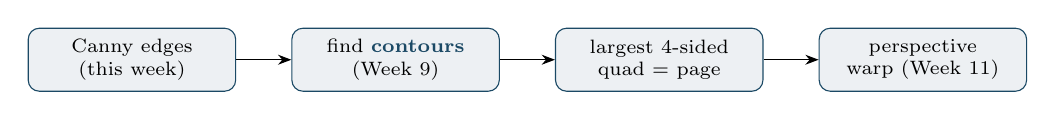
\begin{tikzpicture}[font=\scriptsize,node distance=7mm,
    box/.style={draw=coursePrimary,fill=coursePrimary!8,rounded corners,
      minimum height=8mm,text width=2.4cm,align=center},>=Stealth]
    \node[box](a){Canny edges\\(this week)};
    \node[box,right=of a](b){find \term{contours}\\(Week 9)};
    \node[box,right=of b](c){largest 4-sided\\quad = page};
    \node[box,right=of c](d){perspective\\warp (Week 11)};
    \draw[->](a)--(b);\draw[->](b)--(c);\draw[->](c)--(d);
  \end{tikzpicture}
  \end{center}
  \begin{itemize}
    \item Canny gives the page/meter boundary as connected edges.
    \item Next (Week 9): keep the largest 4-sided contour — the page. Then (Week 11): warp its 4 corners.
  \end{itemize}
  \keyidea{Edges aren't the goal — they're the raw material for finding \emph{shapes} and \emph{structure}.}
\end{frame}

\begin{frame}{What you should now be able to do}
  \begin{itemize}
    \item Explain and trace all four Canny steps (smooth, gradient, NMS, hysteresis).
    \item Run \code{cv2.Canny}, tune the two thresholds, and implement auto-Canny.
    \item Say why NMS thins and why hysteresis connects.
    \item Connect clean edges to the DocScan page-finding pipeline.
  \end{itemize}
\end{frame}

\begin{frame}{This week's deliverable}
  \begin{alertblock}{Due before Week 6 (see \code{project/})}
    \begin{enumerate}
      \item Compute Sobel-x/y and magnitude on a meter; visualize each (Session 1).
      \item Run Canny; show the effect of smoothing (with vs without) and of the two thresholds.
      \item Implement auto-Canny from the median; compare to hand-tuned thresholds.
      \item DocScan: get clean edges of the page/meter boundary on 3 real photos.
    \end{enumerate}
  \end{alertblock}
\end{frame}

\begin{frame}[standout]
  Smooth, differentiate, thin, connect.\\[4pt]
  \normalsize That's Canny — and that's the edge map DocScan will turn into a page.
\end{frame}

\end{document}
